\documentclass{article}

\usepackage[dvips]{graphicx}
\usepackage{color}
\usepackage{boxedminipage}
\usepackage{amsfonts}
\usepackage{amsmath}
\usepackage{url}
\usepackage{caption}
\usepackage{tikz}

\usepackage{Sweave}
\begin{document}
\Sconcordance{concordance:calibration_report.tex:calibration_report.Rnw:%
1 11 1 1 0 8 1 1 6 145 1}


  \title{Calibration Analysis}
	\maketitle
	
	This document lays out all the plots that we want to use in the report.
	
	

\section{Calibration Analysis}
After running all the Latin Hypercube Sampled configurations, we calculated an objective score for each of the configurations to see which ones were better reflecting the real parameters.
  
  \begin{figure}[ht]
		\centering{
		  \textbf{Calibration Results}\par\medskip
			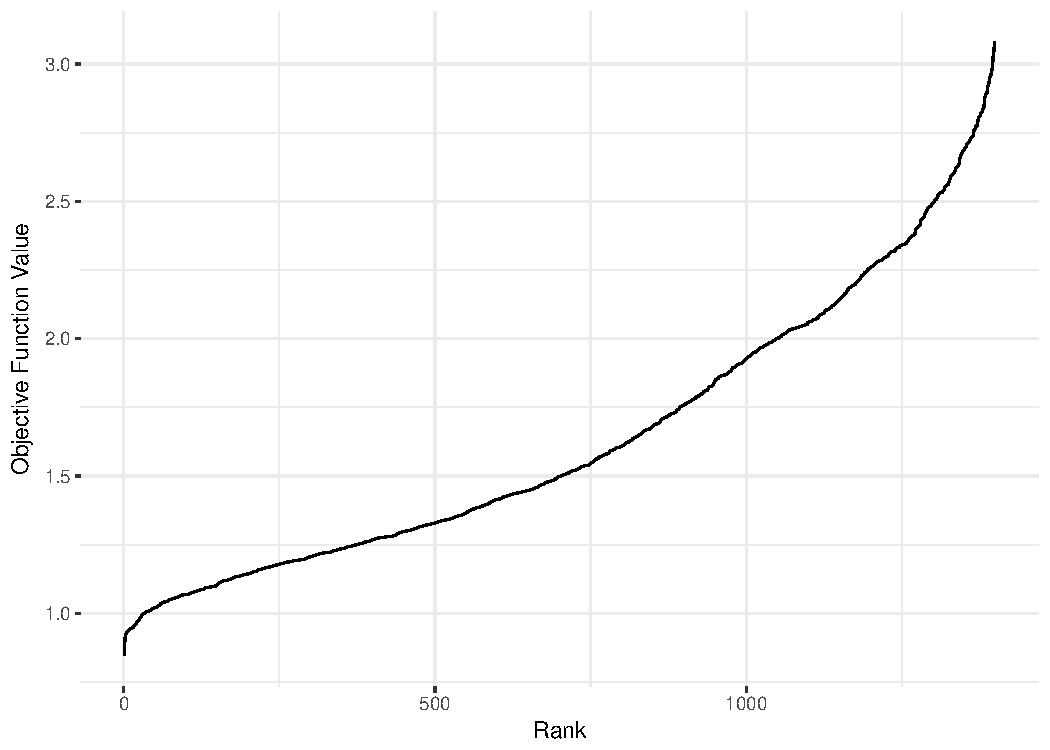
\includegraphics[width=\linewidth]{plots/calibration_results.pdf}
		}
		\caption{Model-Runs Ranked based on their Objective Function Values}
	\end{figure}
	
\section{Sensitivity Results}
For the sensitivity analysis, we used Classification and Regression Trees (CART), Recursive Partitioning and Regression Trees (RPART), and RandomForest techniques. In the analysis of each output against the inputs, we ran analysis of variance (ANOVA) using each technique, and then averaged the resulting values. This average is the composite score on which the following heatmaps are produced.

  \begin{figure}[ht]
		\centering{
		  \textbf{Most Influential Inputs of the Model}\par\medskip
			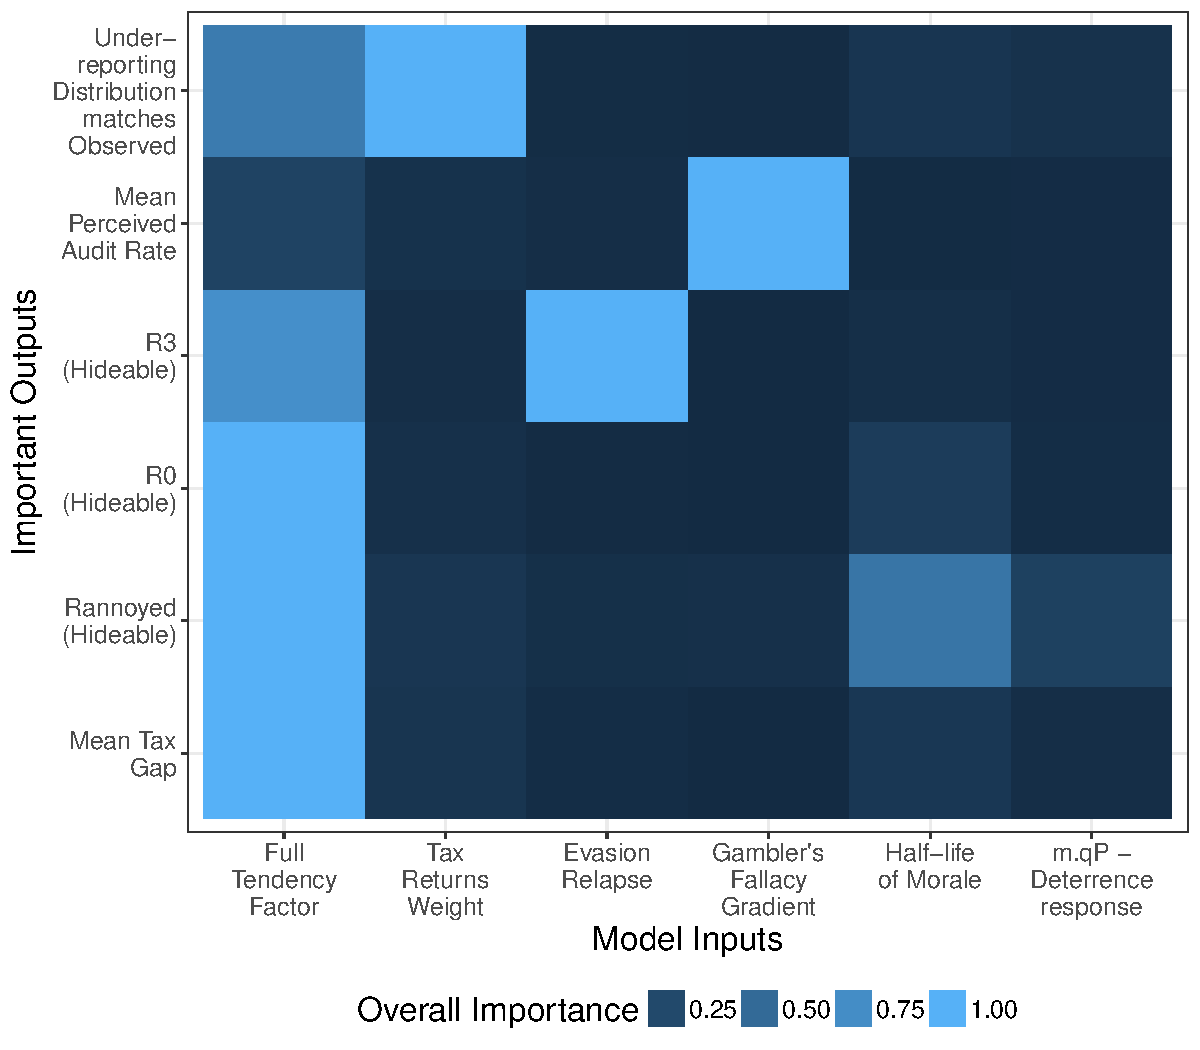
\includegraphics[width=\linewidth]{plots/heatmap_main_outputs.pdf}
		}
		\caption{Heatmap of all Important Outputs against their Most Influential Inputs}
	\end{figure}

  \begin{figure}[ht]
		\centering{
		  \textbf{Other Influential Inputs of the Model}\par\medskip
			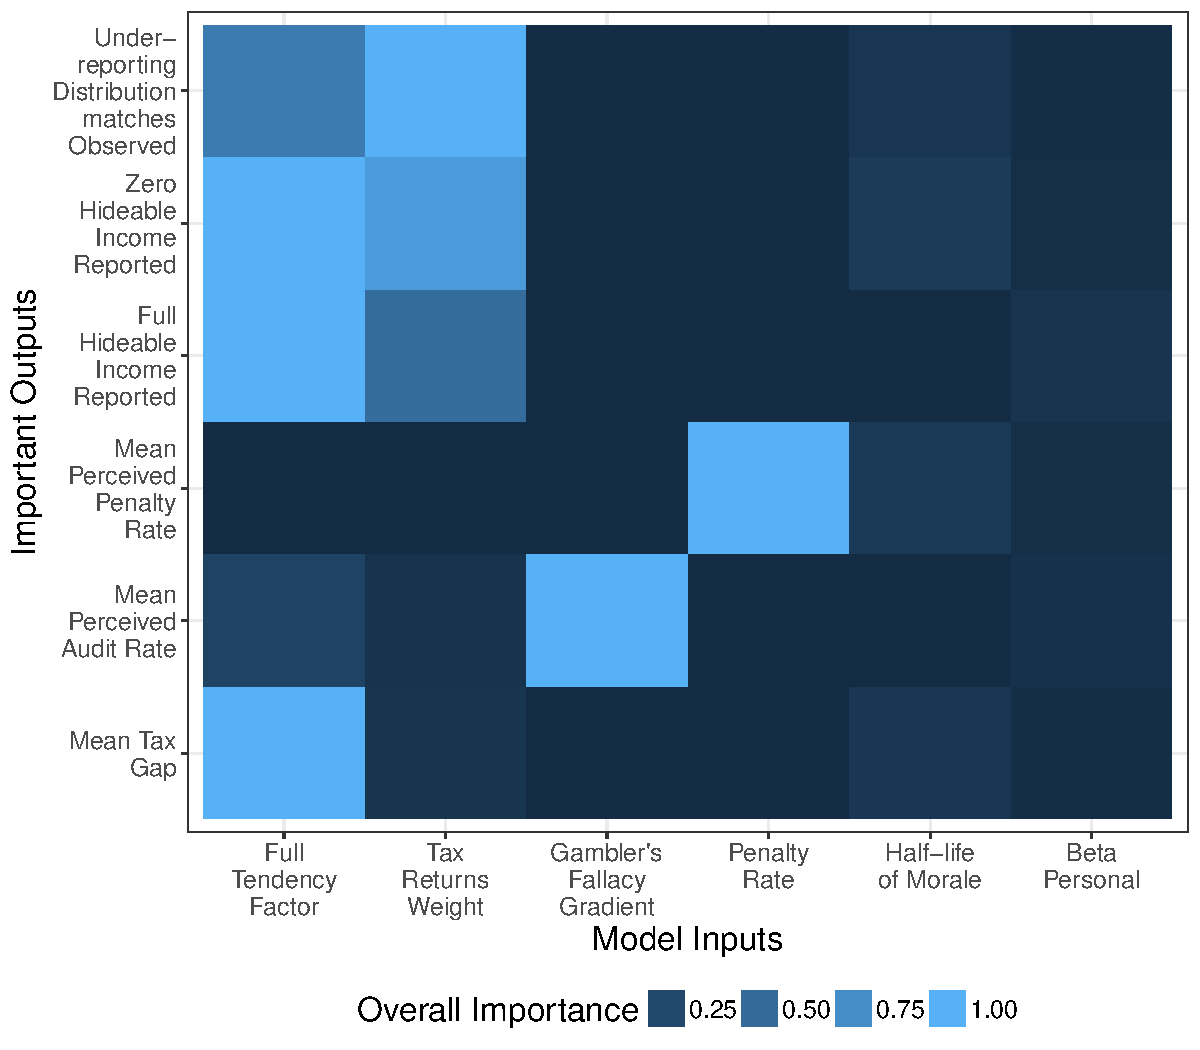
\includegraphics[width=\linewidth]{plots/heatmap_important_R_outputs.pdf}
		}
		\caption{Heatmap of other Important Outputs against their Most Influential Inputs}
	\end{figure}
	
\subsection{Some Tree Outputs}
These RPART plots show what percentage of model-runs are divide the variance of model-outputs in two halves based on the model-inputs at each level. The figure in the middle shows the average predicted value of the output of interest. 

  \begin{figure}[ht]
		\centering{
		  \textbf{Variance of Mean Percieved Audit Rate}\par\medskip
			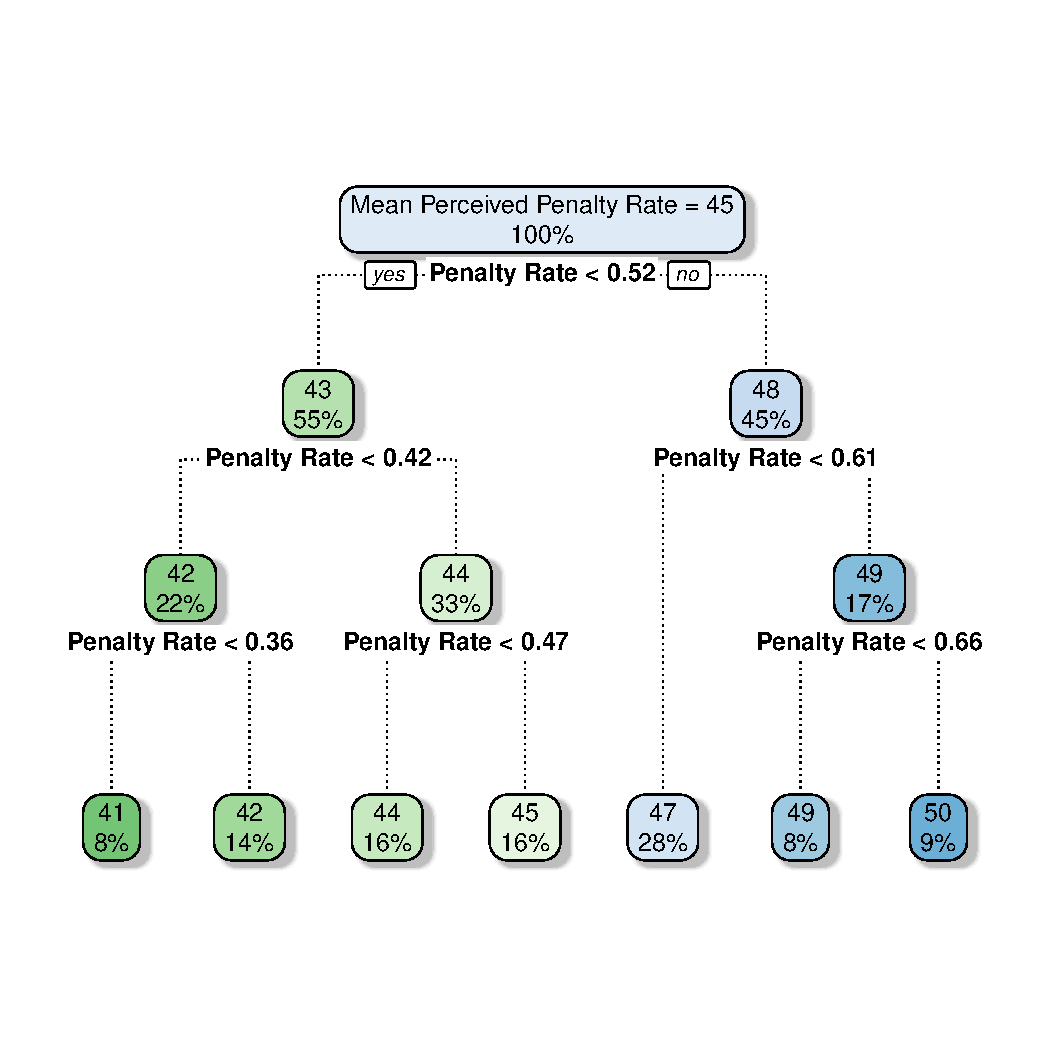
\includegraphics[width=\linewidth]{plots/cart_plot_mean_per_penalty_rate.pdf}
		}
		\caption{RPART Plot of Mean Perceived Penalty Rate}
	\end{figure}
      
  \begin{figure}[ht]
		\centering{
		  \textbf{Variance of Tax Gap}\par\medskip
			\includegraphics[width=\linewidth]{plots/cart_plot_tax_gap_percent.pdf}
		}
		\caption{RPART Plot of Mean Tax Gap}
	\end{figure}
	
\section{Best Case Analysis}
Based on the calibration exercise, we ranked all the model-runs to see which model-run closest reproduces the known parameters. After that was done, we took the best case and here are some interesting outputs of the best case.
\subsection{Aggregate Level Outputs}
Aggregate level outputs are perhaps among the most important outputs of interest for decision makers. The following figures show how tax gap, perceived audit rate, and perceived penalty rate of the simulated population, as a whole, changes over time. Unless otherwise mentioned, all income tax evasion are expressed in terms of hideable income rather than actual income of agents. Hideable income is the percentage of an individual's income that is not expressly known to the tax authorities. Self employed individuals, in general, have a higher hideable income than non-self-employed individuals due to appropriate reporting mechanisms in place. 
  \begin{figure}[ht]
		\centering{
		  \textbf{Aggregate Outputs}\par\medskip
			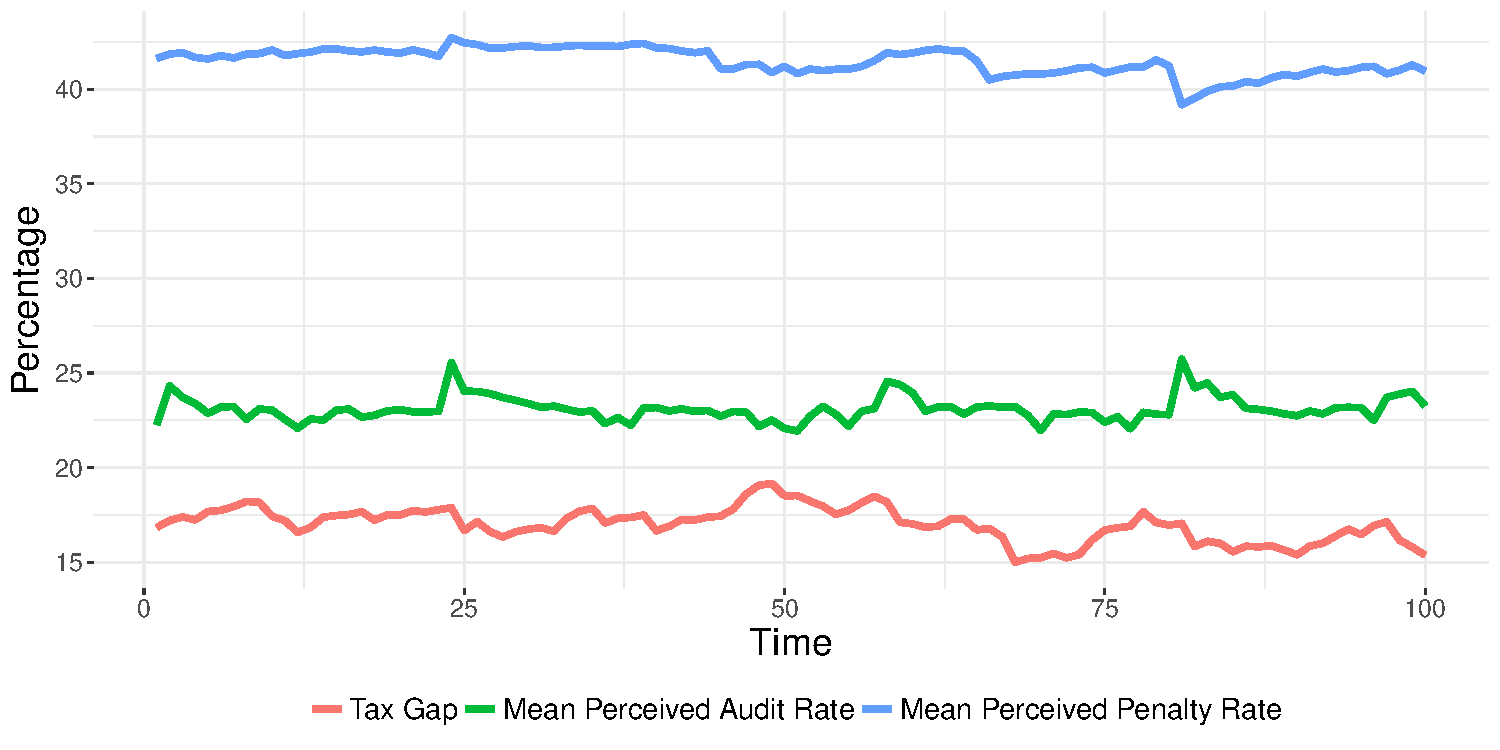
\includegraphics[width=\linewidth]{plots/Model_aggregated_dyn_plot.pdf}
		}
		\caption{Aggregate Outputs of the Best Case}
	\end{figure}
	
	\begin{figure}[ht]
		\centering{
		  \textbf{Iterative Plot of Tax Gap}\par\medskip
			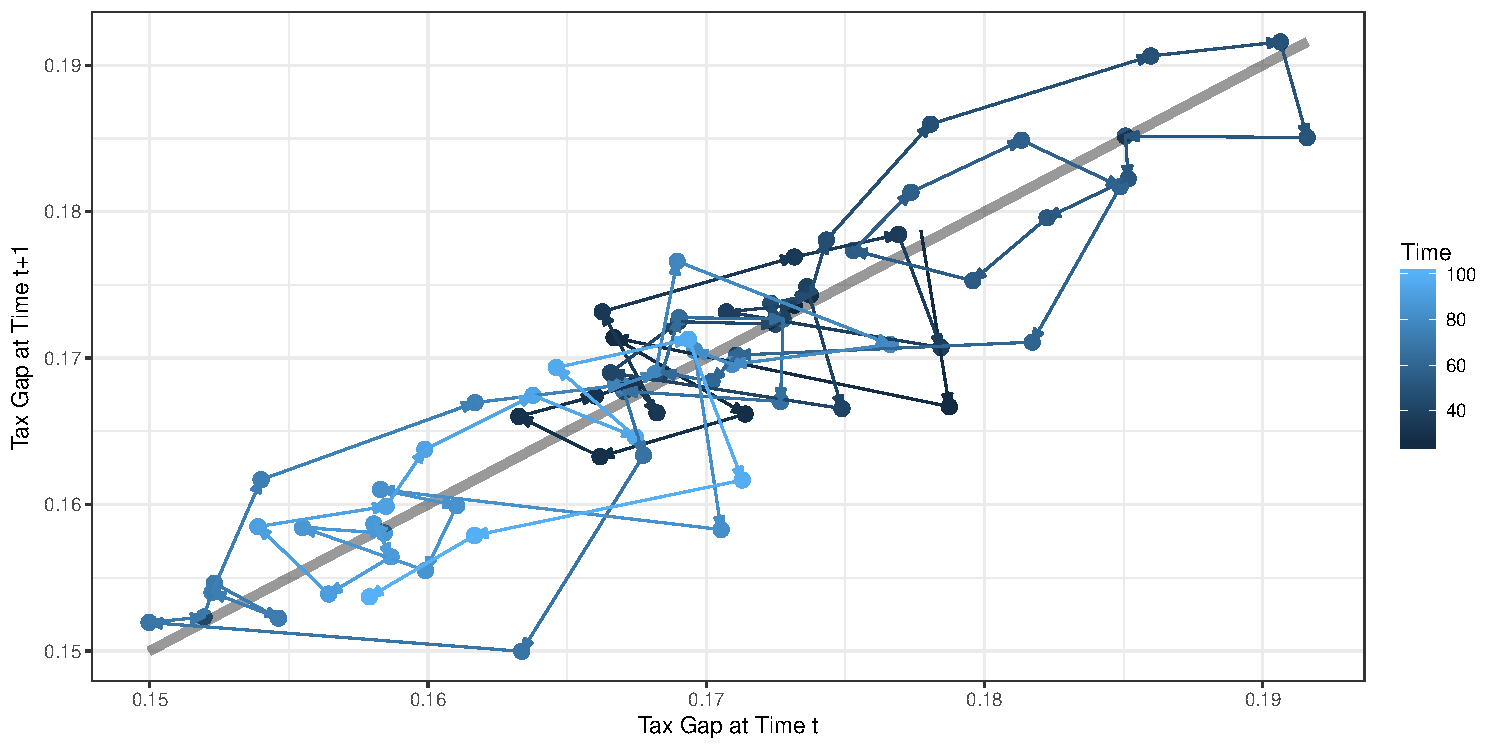
\includegraphics[width=\linewidth]{plots/Model_iterative_map_plot.pdf}
		}
		\caption{Iterative Plot Showing how Tax Gap Varies from One Year to the Next}
	\end{figure}

\subsection{Individual Level Outputs}
While the above plots were aggreagate level outputs, the more interesting plots are the ones that show individual trajectories. Here are a few plots showing the behavior of individuals grouped by their employment status (self-employed or non-sel-employed). Self-employed individuals are known to have more opportunities to evade taxes, than non-self-employed people.These plots show how much of the hideable income to agents report. 

  \begin{figure}[ht]
		\centering{
		  \textbf{Selected Trajectories of Self-Employed Agents}\par\medskip
			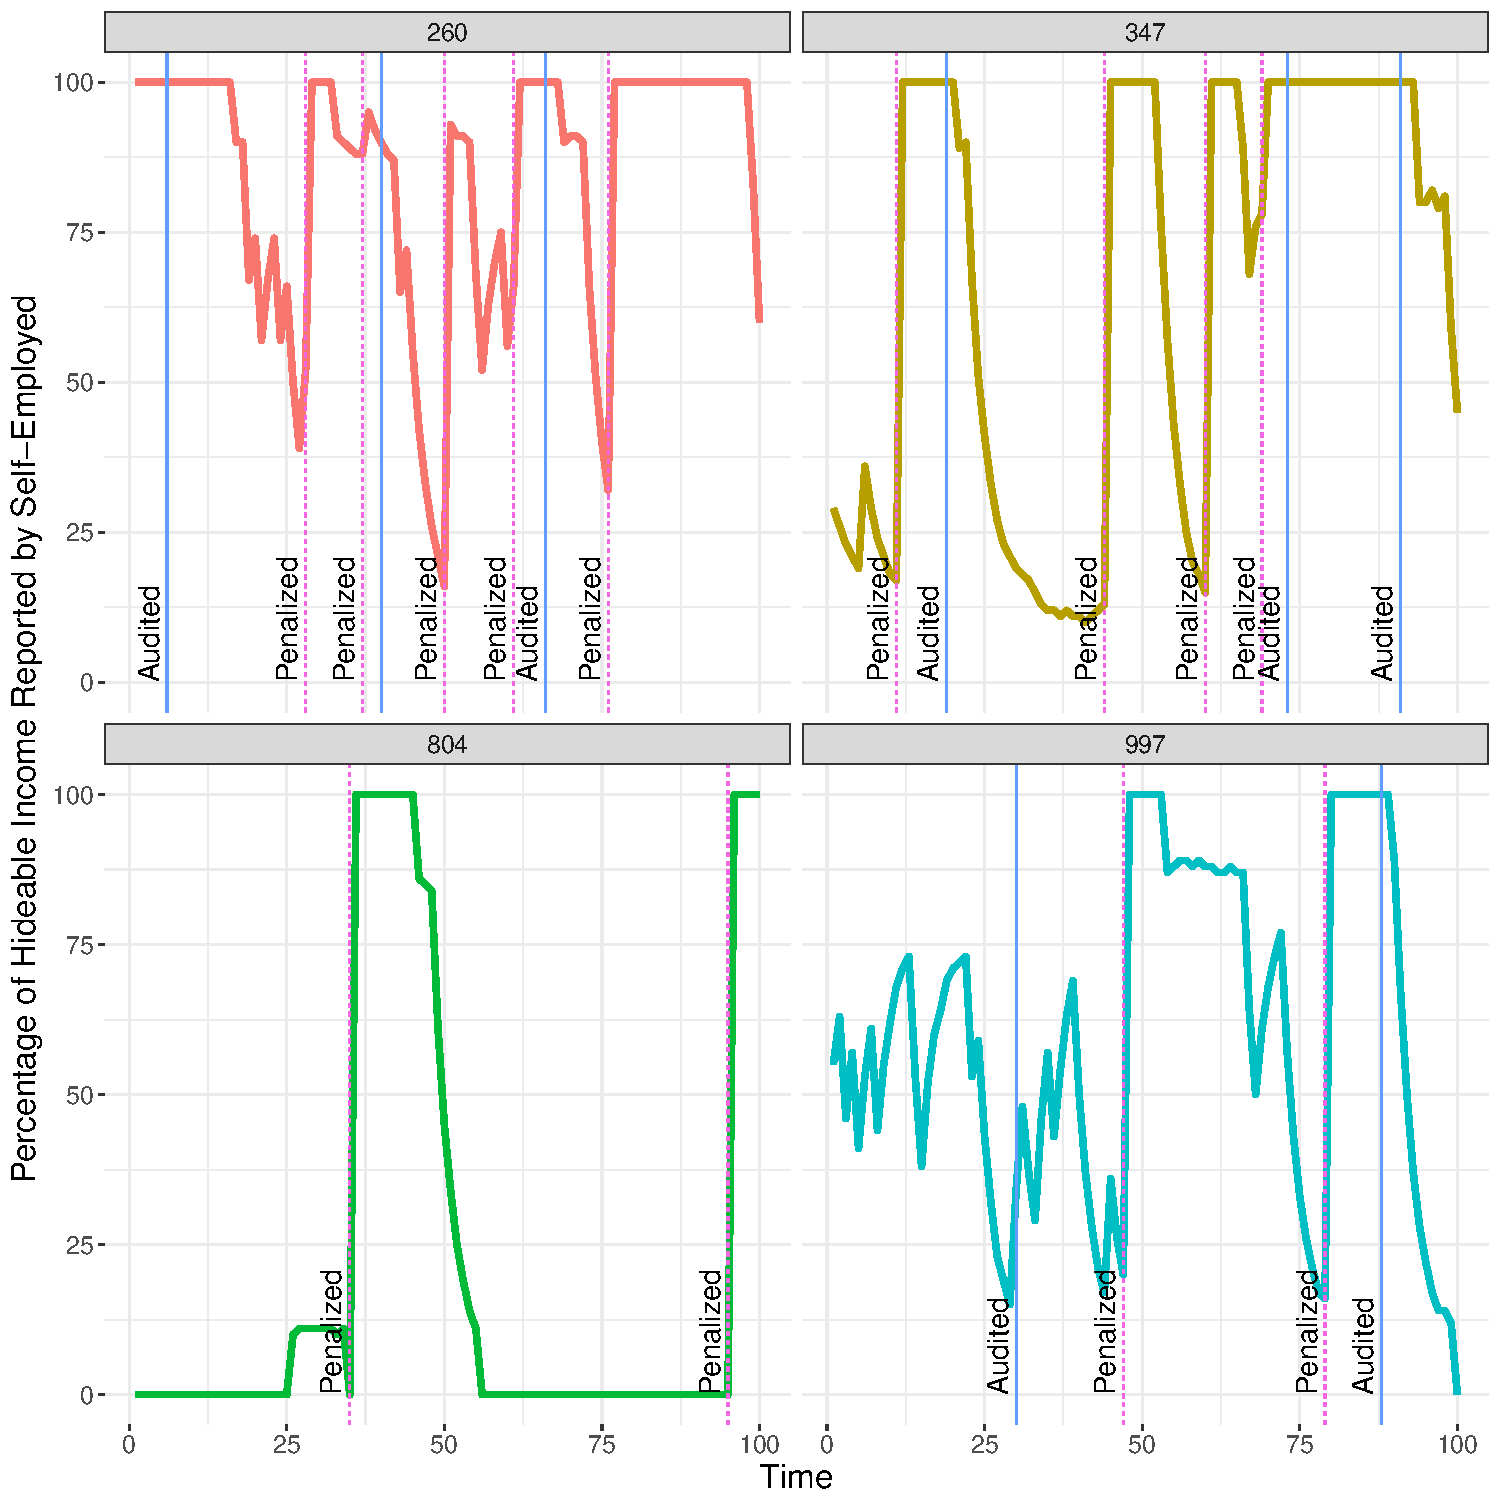
\includegraphics[width=\linewidth]{plots/Model_se_trajectory_plot.pdf}
		}
		\caption{Individual Trajectories showing Hideable Income Reported by a few Self-Employed Agents}
	\end{figure}
	
	
  \begin{figure}[ht]
		\centering{
		  \textbf{Selected Trajectories of Non-Self-Employed Agents}\par\medskip
			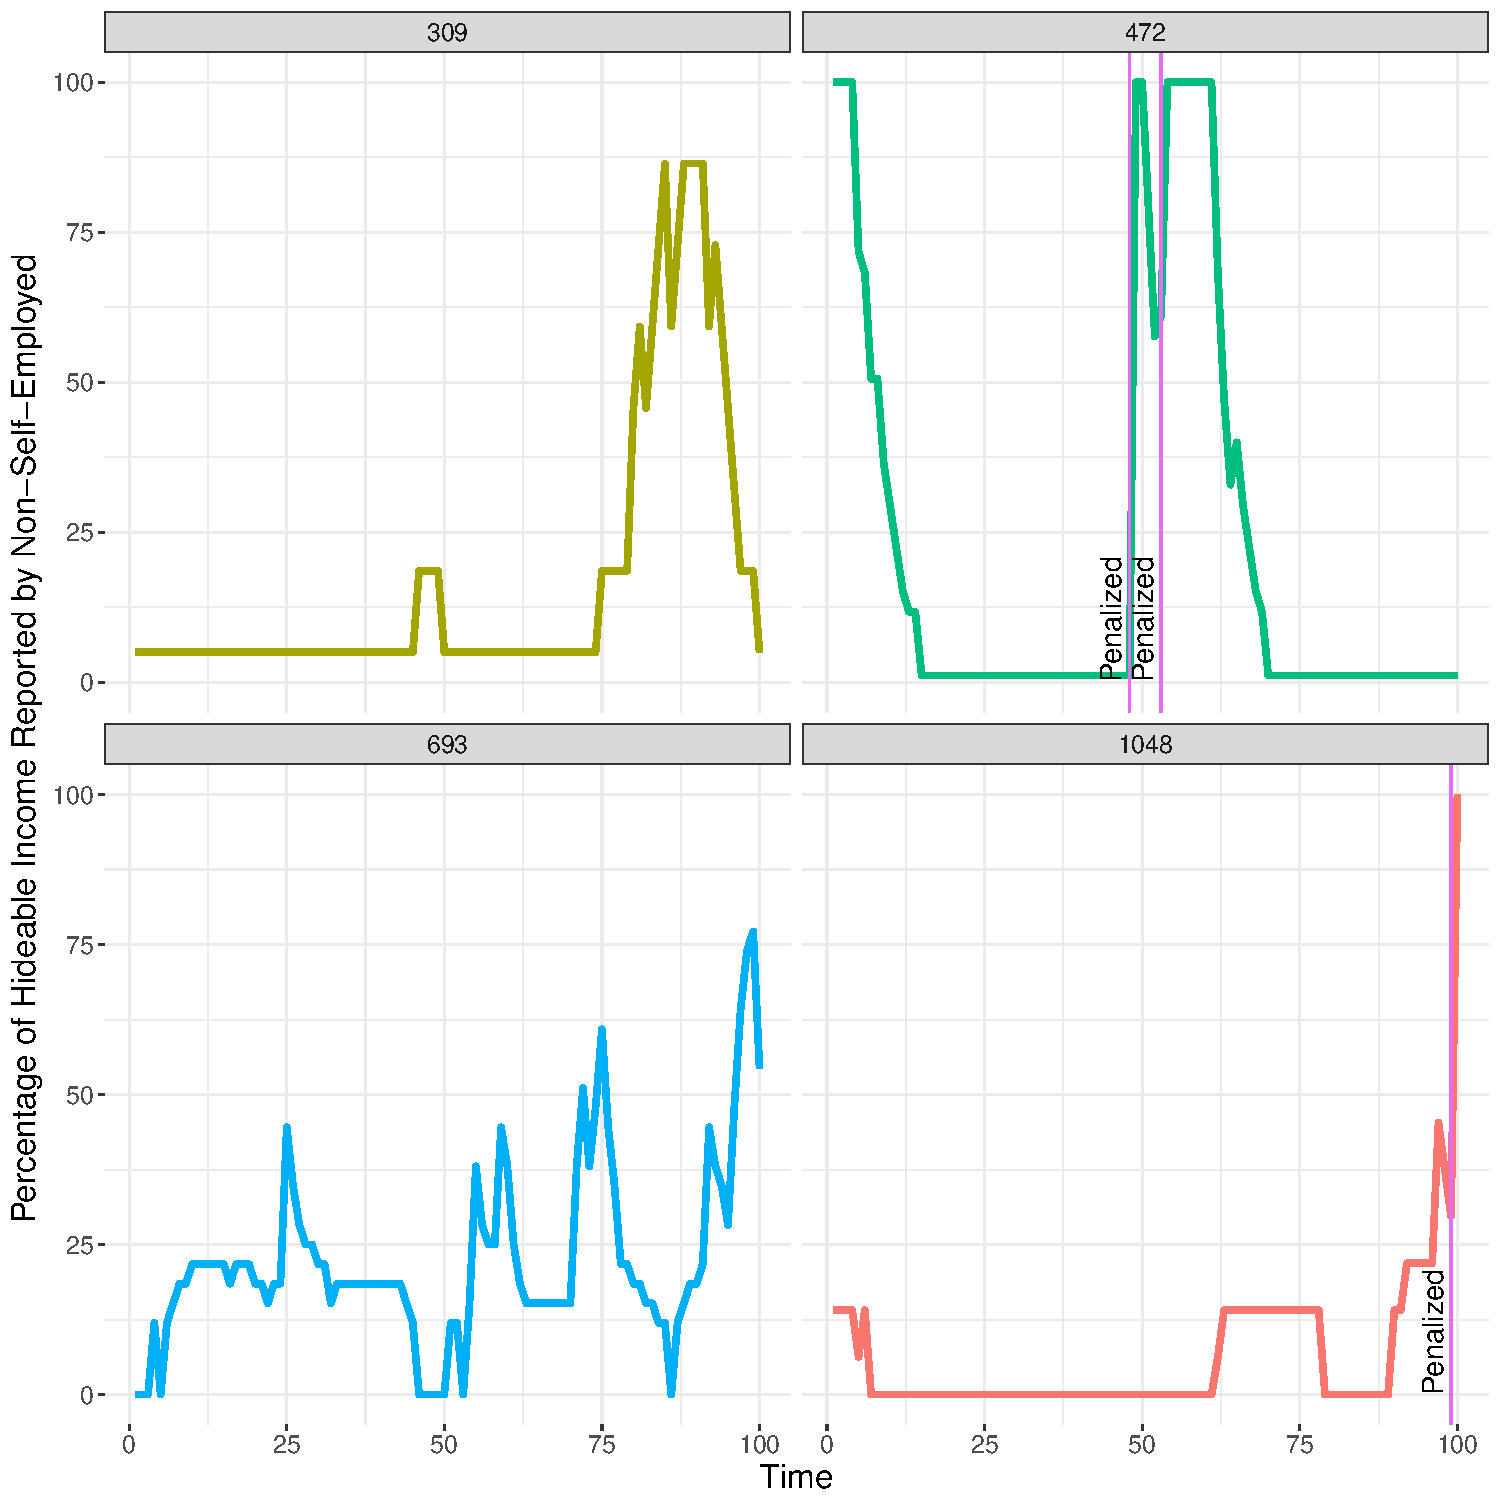
\includegraphics[width=\linewidth]{plots/Model_nse_trajectory_plot.pdf}
		}
		\caption{Individual Trajectories showing Hideable Income Reported by a few Non-Self-Employed Agents}
	\end{figure}
	
\subsection{Population Distributions}
Now that we have seen aggregate level outputs and individual behaviors, here are a few plots examinng the distribution of outputs among the simulated population. 	
  
  \begin{figure}[ht]
		\centering{
		  \textbf{Hideable Income Reporting Distribution}\par\medskip
			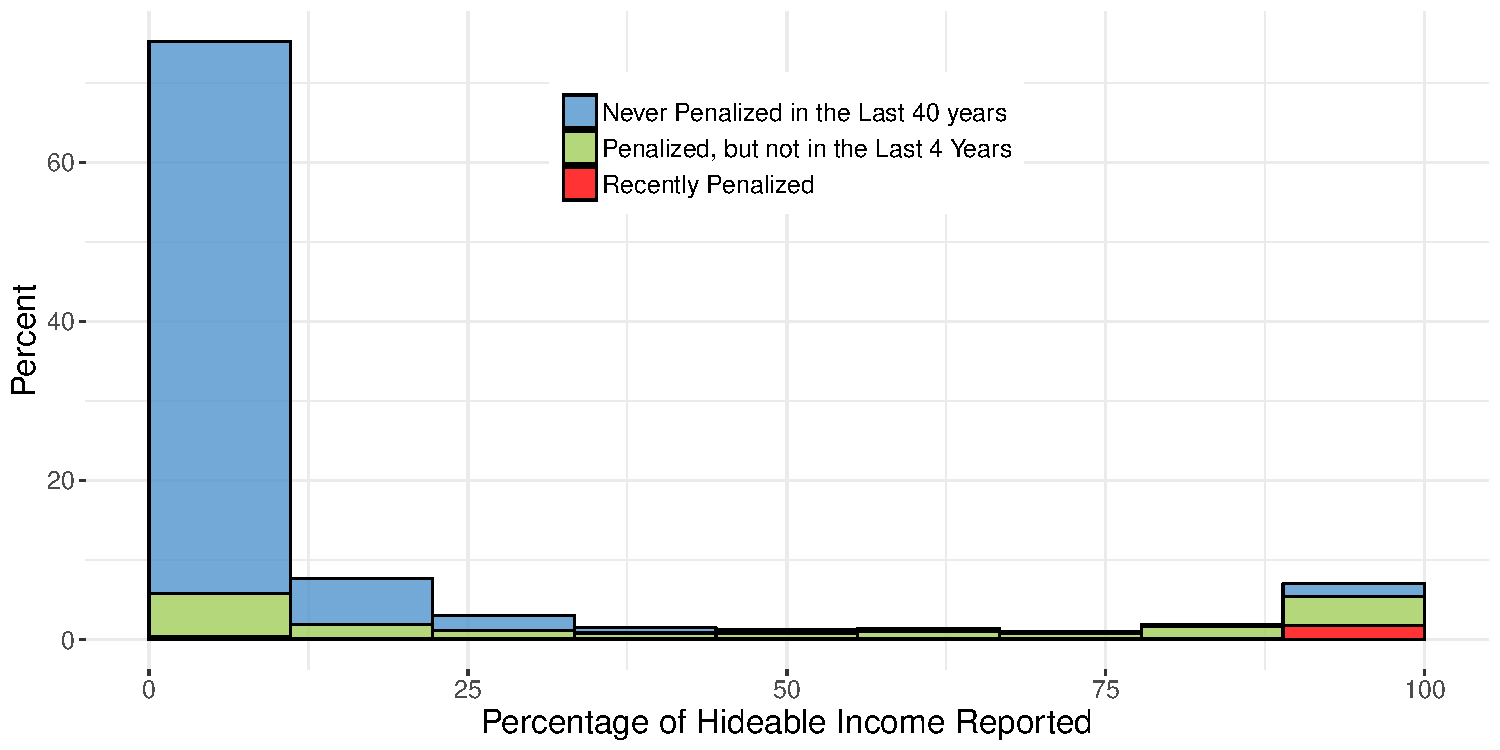
\includegraphics[width=\linewidth]{plots/Model_report_plot.pdf}
		}
		\caption{Distribution of how Hideable Income is Reported by Agents}
	\end{figure}
	
	\begin{figure}[ht]
		\centering{
		  \textbf{Percieved Audit Rate Distribution}\par\medskip
			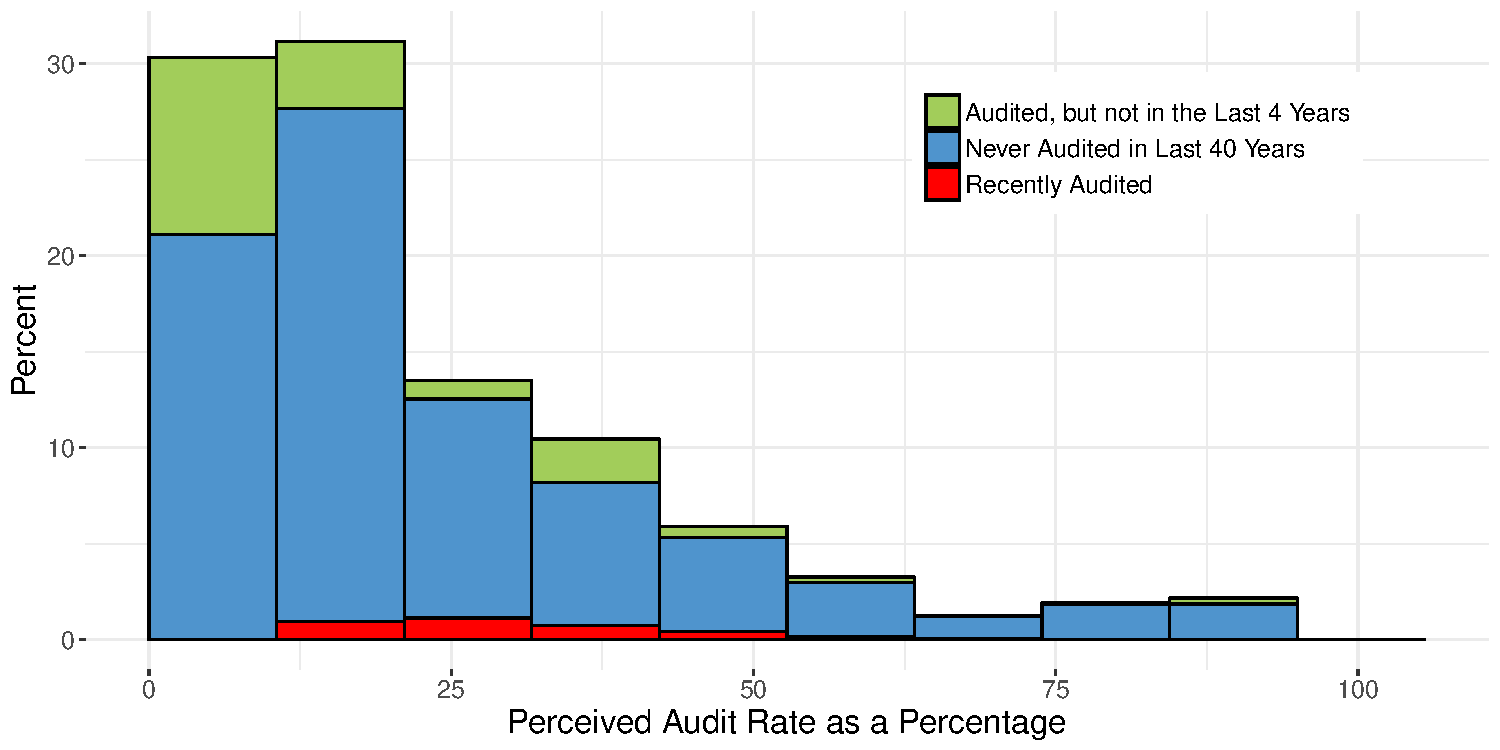
\includegraphics[width=\linewidth]{plots/Model_per_audit_rate_plot.pdf}
		}
		\caption{Distribution of Perceived Audit Rate of Agents}
	\end{figure}
	
	\begin{figure}[ht]
		\centering{
		  \textbf{Percieved Penalty Rate Distribution}\par\medskip
			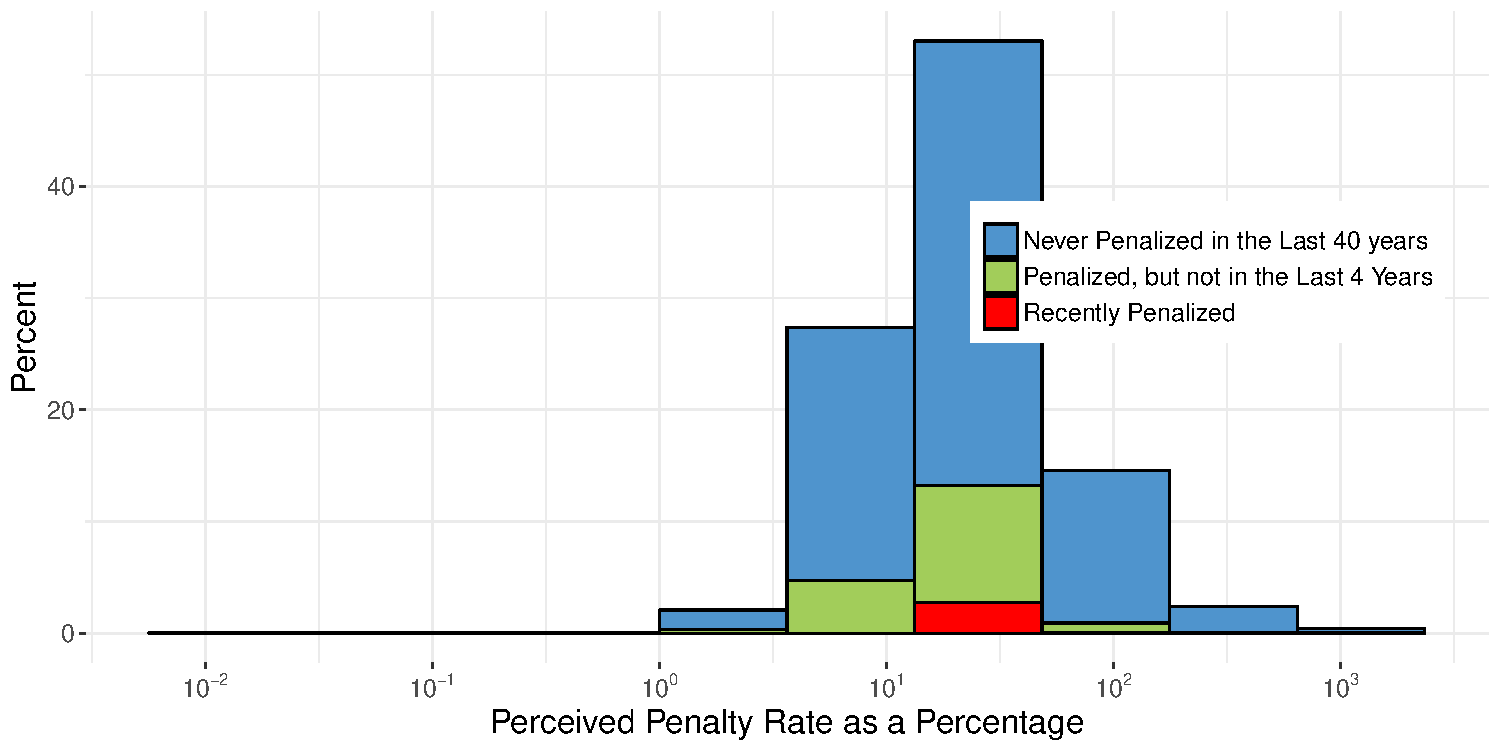
\includegraphics[width=\linewidth]{plots/Model_per_penalty_rate_plot.pdf}
		}
		\caption{Distribution of Perceived Penalty Rate of Agents}
	\end{figure}
	
	\begin{figure}[ht]
		\centering{
		  \textbf{Distribution of Compliance}\par\medskip
			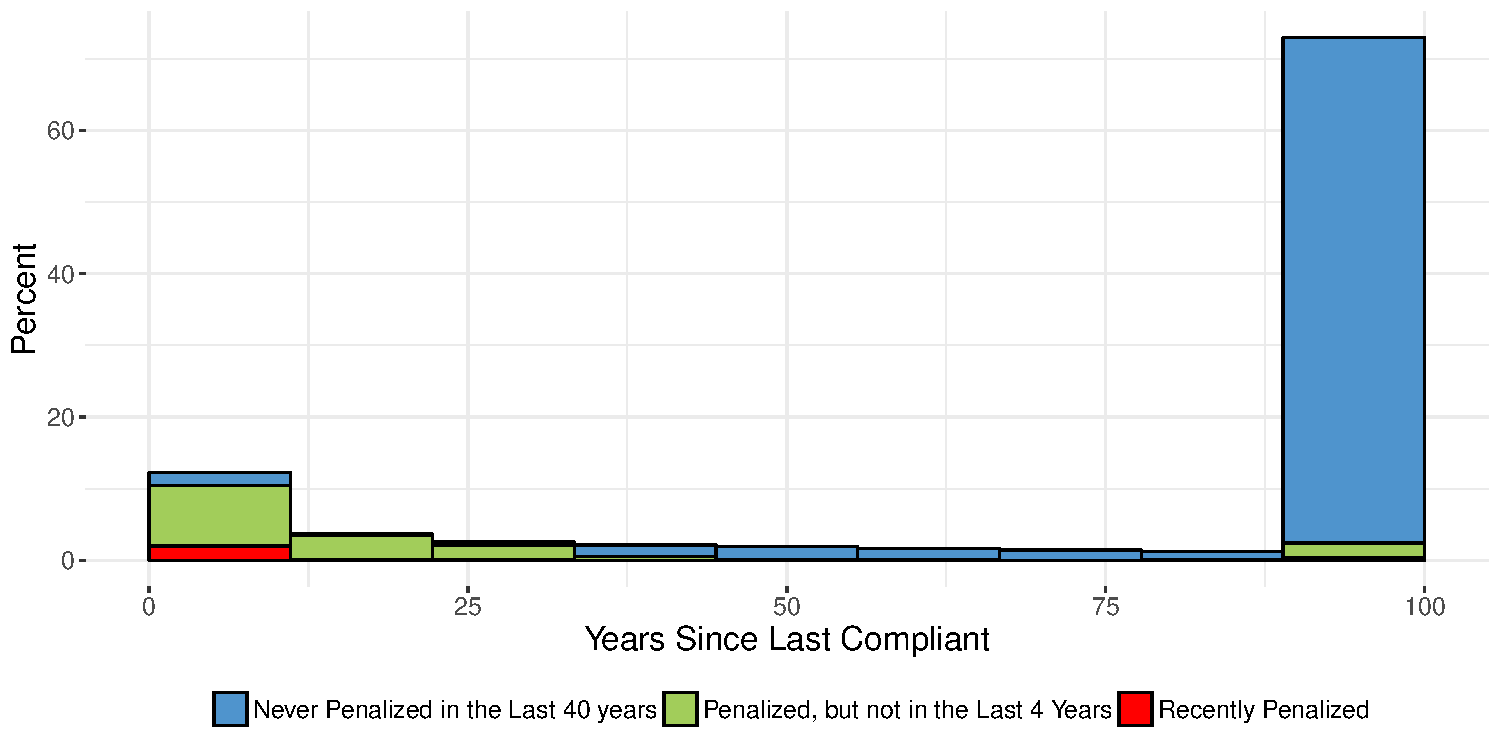
\includegraphics[width=\linewidth]{plots/Model_years_since_last_compliant_plot.pdf}
		}
		\caption{Distribution of Compliance Behavior of Agents Over Time}
	\end{figure}
	
	\begin{figure}[ht]
		\centering{
		  \textbf{Propensity to Fully Report Income}\par\medskip
			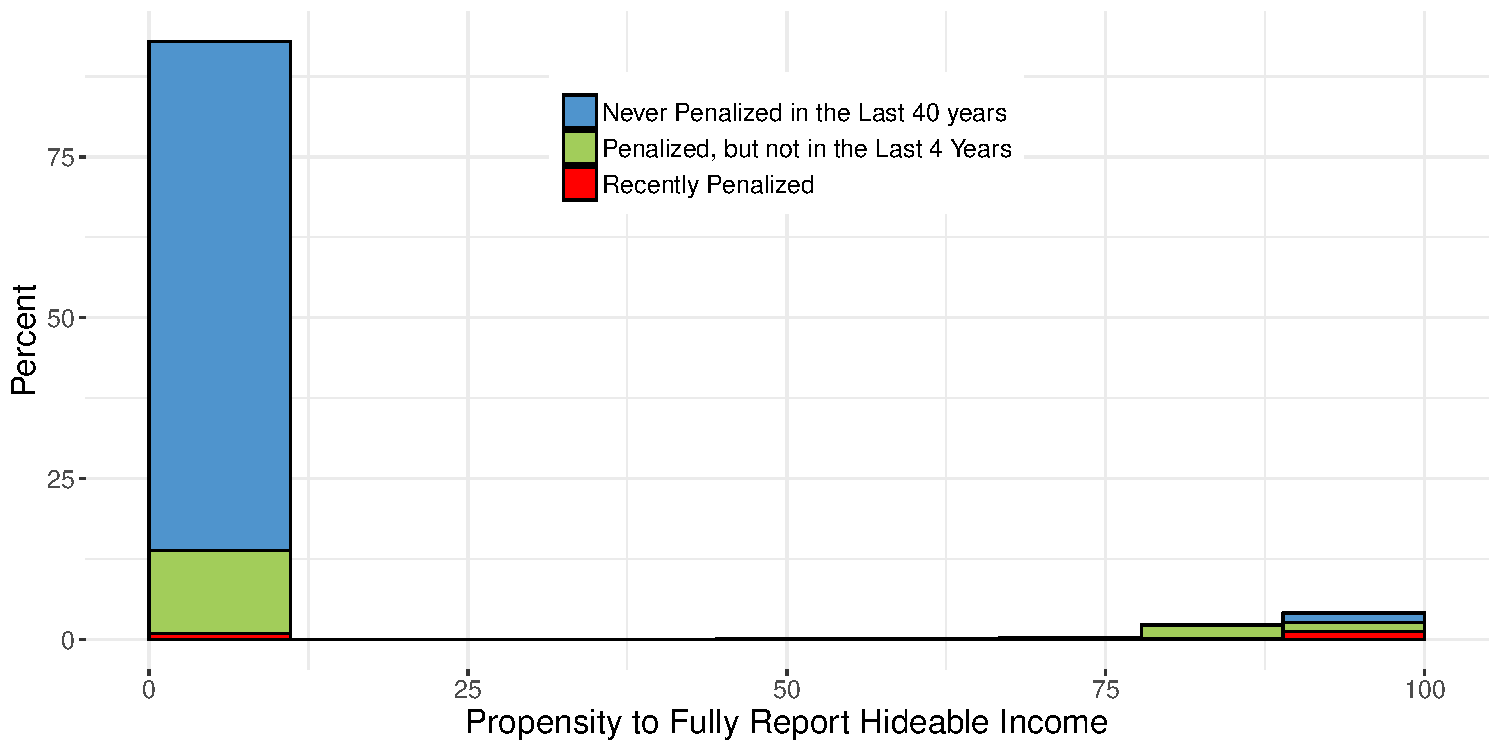
\includegraphics[width=\linewidth]{plots/Model_w_plot.pdf}
		}
		\caption{Distribution showing the Propensity of Agents to Report All of their Income}
	\end{figure}
	
	\begin{figure}[ht]
		\centering{
		  \textbf{c1 and c2}\par\medskip
			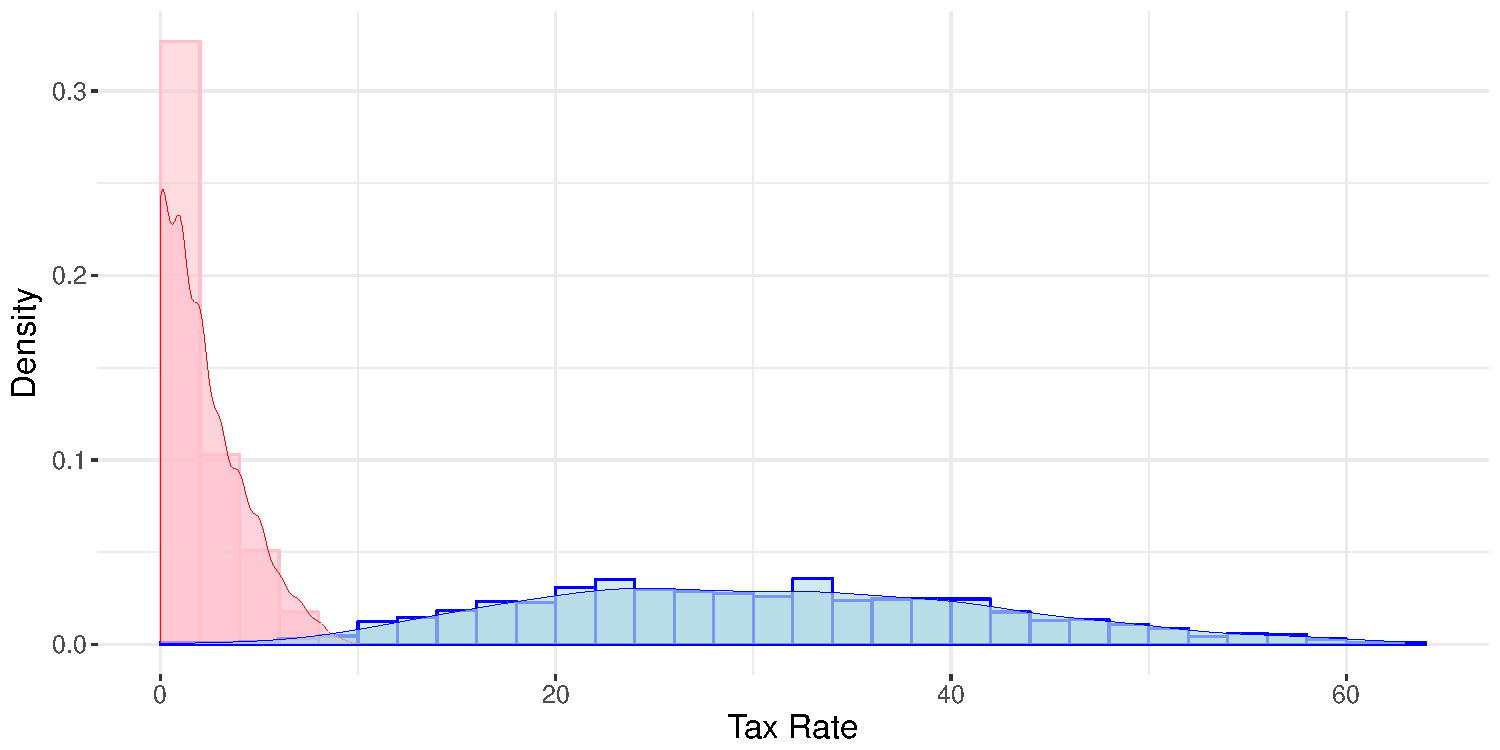
\includegraphics[width=\linewidth]{plots/Model_c1_plot.pdf}
		}
		\caption{Distribution of c1 and c2 Thresholds of the Agents}
	\end{figure}
	
	
	

\end{document}

